% !TeX spellcheck = en_US
%% 
%% Copyright 2007-2020 Elsevier Ltd
%% 
%% This file is part of the 'Elsarticle Bundle'.
%% ---------------------------------------------
%% 
%% It may be distributed under the conditions of the LaTeX Project Public
%% License, either version 1.2 of this license or (at your option) any
%% later version.  The latest version of this license is in
%%    http://www.latex-project.org/lppl.txt
%% and version 1.2 or later is part of all distributions of LaTeX
%% version 1999/12/01 or later.
%% 
%% The list of all files belonging to the 'Elsarticle Bundle' is
%% given in the file `manifest.txt'.
%% 
%% Template article for Elsevier's document class `elsarticle'
%% with harvard style bibliographic references

%\documentclass[preprint,12pt,authoryear]{elsarticle}

%% Use the option review to obtain double line spacing
%% \documentclass[authoryear,preprint,review,12pt]{elsarticle}

%% Use the options 1p,twocolumn; 3p; 3p,twocolumn; 5p; or 5p,twocolumn
%% for a journal layout:
%% \documentclass[final,1p,times,authoryear]{elsarticle}
%% \documentclass[final,1p,times,twocolumn,authoryear]{elsarticle}
%% \documentclass[final,3p,times,authoryear]{elsarticle}
%% \documentclass[final,3p,times,twocolumn,authoryear]{elsarticle}
%% \documentclass[final,5p,times,authoryear]{elsarticle}
 \documentclass[final,5p,times,twocolumn,authoryear]{elsarticle}

%% For including figures, graphicx.sty has been loaded in
%% elsarticle.cls. If you prefer to use the old commands
%% please give \usepackage{epsfig}

%% The amssymb package provides various useful mathematical symbols
\usepackage{amssymb}
\usepackage{lipsum}
%% The amsthm package provides extended theorem environments
%% \usepackage{amsthm}

%% The lineno packages adds line numbers. Start line numbering with
%% \begin{linenumbers}, end it with \end{linenumbers}. Or switch it on
%% for the whole article with \linenumbers.
%% \usepackage{lineno}

%% You might want to define your own abbreviated commands for common used terms, e.g.:
\newcommand{\kms}{km\,s$^{-1}$}
\newcommand{\msun}{$M_\odot}

\journal{Dr. Amin Faraji}


\begin{document}

\begin{frontmatter}

%% Title, authors and addresses

%% use the tnoteref command within \title for footnotes;
%% use the tnotetext command for theassociated footnote;
%% use the fnref command within \author or \affiliation for footnotes;
%% use the fntext command for theassociated footnote;
%% use the corref command within \author for corresponding author footnotes;
%% use the cortext command for theassociated footnote;
%% use the ead command for the email address,
%% and the form \ead[url] for the home page:
%% \title{Title\tnoteref{label1}}
%% \tnotetext[label1]{}
%% \author{Name\corref{cor1}\fnref{label2}}
%% \ead{email address}
%% \ead[url]{home page}
%% \fntext[label2]{}
%% \cortext[cor1]{}
%% \affiliation{organization={},
%%            addressline={}, 
%%            city={},
%%            postcode={}, 
%%            state={},
%%            country={}}
%% \fntext[label3]{}

\title{Exploring Periodic Boundary Conditions: A Study on 2D and 3D Spheres and Continuum Limit}

%% use optional labels to link authors explicitly to addresses:
%% \author[label1,label2]{}
%% \affiliation[label1]{organization={},
%%             addressline={},
%%             city={},
%%             postcode={},
%%             state={},
%%             country={}}
%%
%% \affiliation[label2]{organization={},
%%             addressline={},
%%             city={},
%%             postcode={},
%%             state={},
%%             country={}}

\author[first]{Alireza Same}
\fntext[first]{99100709}
\ead{alirezasame@gmail.com}
\author[second]{Hanie Hatami}
\fntext[second]{99100614}
\ead{alirezasame@gmail.com}
\author[third]{Mehrnaz Rabiee}
\fntext[third]{99100669}
\ead{alirezasame@gmail.com}

\begin{abstract}
%% Text of abstract
We analyze systems with periodic boundary conditions in two and three dimensions. Beginning with an $N$-particle system confined to a circle, we derive the governing ordinary differential equation and solve it both analytically using circulant matrices and numerically. We then take the continuum limit as $N$ goes to infinity to obtain a wave equation on the circle with periodic boundary conditions. This partial differential equation is solved exactly, allowing us to construct visualizations of the propagating waves. Next we study an $N$-particle system confined to the surface of a regular polyhedron, deriving the discrete equations and solving numerically using symmetry arguments. We then discuss statistical mechanics approaches for this system. Finally, we analyze longitudinal elastic waves propagating on a sphere, deriving the continuum wave equation in spherical coordinates and discussing analytical and numerical solution methods based on spectral decomposition. Throughout we emphasize the mathematical physics, solving equations analytically where possible and numerically otherwise. Results for all systems are illustrated through figures.
\end{abstract}

%%Graphical abstract
%\begin{graphicalabstract}
%\includegraphics{grabs}
%\end{graphicalabstract}

%%Research highlights
%\begin{highlights}
%\item Research highlight 1
%\item Research highlight 2
%\end{highlights}

\begin{keyword}
%% keywords here, in the form: keyword \sep keyword, up to a maximum of 6 keywords
Particle Systems \sep Mathematical Physics \sep Fourier Analysis \sep Differential Equations \sep Continuum Limit \sep Periodic Symmetry \sep Platonic Solids

%% PACS codes here, in the form: \PACS code \sep code

%% MSC codes here, in the form: \MSC code \sep code
%% or \MSC[2008] code \sep code (2000 is the default)

\end{keyword}


\end{frontmatter}

%\tableofcontents

%% \linenumbers

%% main text

\section{Introduction}
\label{introduction}
Periodic boundary conditions arise naturally in the study of waves and particles constrained to closed topologies. The mathematics of such systems, though conceptually simple, reveals rich physical behaviors. In one dimension, systems with periodic boundaries can be solved exactly, yielding insights into phenomena from quantum mechanics to elasticity. As the dimension increases, new challenges emerge. On a circle, the topology is uniform and easily parametrized, yielding to straightforward analysis via Fourier decomposition. On a sphere, the additional dimension introduces variability in the surface curvature, requiring more advanced methods like spherical harmonics. In three dimensions, modeling particles or waves constrained to regular convex polyhedra brings deeper obstacles, as these Platonic solids resist exact geometric parameterization.

Approximation methods must therefore complement exact mathematical techniques in exploring these systems. The interplay of analytical, numerical, and geometric ideas is what makes periodic systems fascinating to study. When symmetry allows clean solutions, the mathematics elegantly explains the physics. And when intricacies of higher dimensions obstruct analysis, numerical methods and geometric intuition guide the way.

In this Article, we embark on a mathematical tour of periodic boundaries in multiple dimensions. We begin with approachable problems, deriving and solving ordinary differential equations through matrix techniques. Moving to continuous systems, we encounter tractable partial differential equations which yield to Fourier analysis. Finally, we contend with intricate geometries, wrestling with equations which only numerical computation can conquer. What ties these investigations together is the quest to understand systems constrained to live within themselves, endowed with a symmetry as beautiful as it is challenging.

\section{2D Spheres Revisited}
\label{sec-2D}
As established in foundational texts on wave phenomena (see \cite{georgiPhysicsWaves2015}), a prototypical model for cyclic wave propagation considers a discrete set of point particles confined to a circular domain. This framework relies on two key approximations: first, that interactions are strictly local, with each particle only directly influencing its immediate neighbors. Second, that the interparticle forces respond linearly to changes in separation relative to an equilibrium length. While undeniably reductionist, these assumptions prove sufficient to capture the salient physics of transverse wave transmission through the medium.

Specifically, we examine a system of N identical particles of mass m regularly spaced around a ring of radius R. Identical harmonic springs, characterized by force constant k, link adjacent particles along the circumference. This geometry exhibits a continuous rotational symmetry - rotations by 2pi/N map the configuration onto itself. Our theoretical description should therefore not differentiate between the 2N symmetry-equivalent orientations. The sole measurable degree of freedom lies in the particles' relative displacements, as absolute positions along the circle can not be experimentally determined without first arbitrarily fixing a reference point.

The simplicity of this model, alongside its inherent periodicity, motivate its study before tackling more intricate geometries in higher dimensions. Even within the confines of localized, linear interactions, analytical and computational techniques reveal rich wave behaviors arising from the cyclic topology. The mathematics provides profound and elegant insight into the underlying physics.

As an elementary example, Figure 1 illustrates the case for N=4 particles. The fourfold rotational symmetry is evident, as is the periodic nature of the circular boundary. With the model established, we now embark on an in-depth analysis.

\begin{figure}
	\centering 
	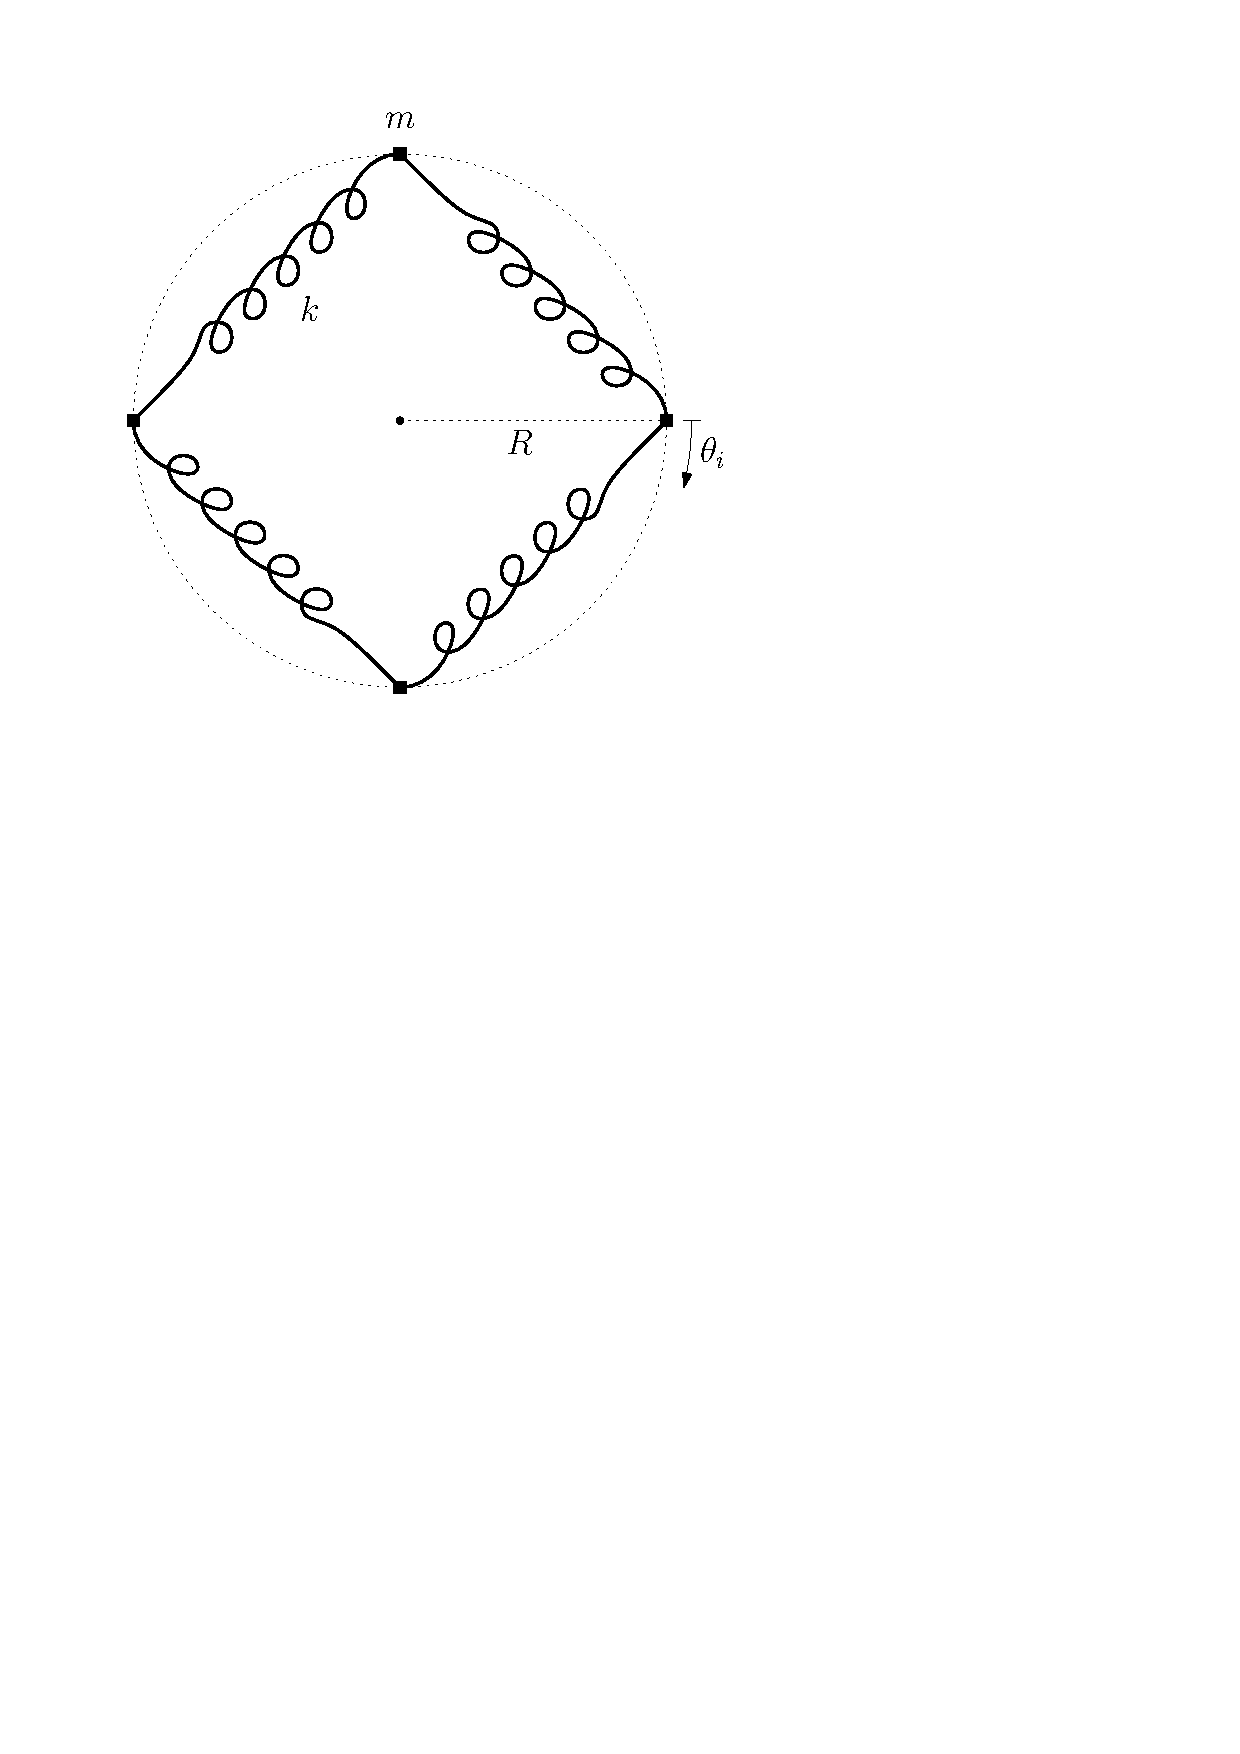
\includegraphics[width=0.25\textwidth]{../Figures/1D-4Particle-Springs.pdf}	
	\caption{4 identically distributed point masses on a circle} 
	\label{fig-n4}
\end{figure}




\section{Discussion}
%%\label{}

\section{Summary and conclusions}
%%\label{}


\section*{Acknowledgements}
Thanks to ...

%% The Appendices part is started with the command \appendix;
%% appendix sections are then done as normal sections

%% If you have bibdatabase file and want bibtex to generate the
%% bibitems, please use
%%
\bibliographystyle{elsarticle-harv} 
\bibliography{zotero}

%% else use the following coding to input the bibitems directly in the
%% TeX file.

%%\begin{thebibliography}{00}

%% \bibitem[Author(year)]{label}
%% For example:

%% \bibitem[Aladro et al.(2015)]{Aladro15} Aladro, R., Martín, S., Riquelme, D., et al. 2015, \aas, 579, A101


%%\end{thebibliography}

\end{document}

\endinput
%%
%% End of file `elsarticle-template-harv.tex'.
